% %%%%%%%%%%%%%%%%%%%%%%%%%%%%%%%%%%%%%%%%%%%%%%%%%%%%%%%%%%%%%%%%%%%%%
% %% State-of-the-Art %%
% SPiDRE
% %%%%%%%%%%%%%%%%%%%%%%%%%%%%%%%%%%%%%%%%%%%%%%%%%%%%%%%%%%%%%%%%%%%%%

\subsection{SPiDRE}
\label{sec:soa:spidre}

The authors of SPiDRE~\cite{Barredo2019_SPiDRE} observed that the main limitation in system performance is the memory latency, especially for sparse data applications where caches became inefficient. Thus, SPiDRE is an accelerator designed to realize near memory sparse to dense conversion, allowing the memory hierarchy to benefit from good data locality.

SPiDRE has a simple architecture that convert in parallel data fetched from main memory and write them back in a compressed format. It is programmable and can be used for many different applications. For example, with a SpMSpM kernel, sparse input matrices could be rearranged through a user defined function to a dense format where all non-zero elements are in the right order of computation. SPiDRE also performs direct virtual-to-physical address translation to reduce area overhead, and maintains memory consistency to avoid read and write conflicts with the host core. Moreover, SPiDRE can easily be scaled to several instances for a higher conversion throughput.

\begin{figure}
    \centering
    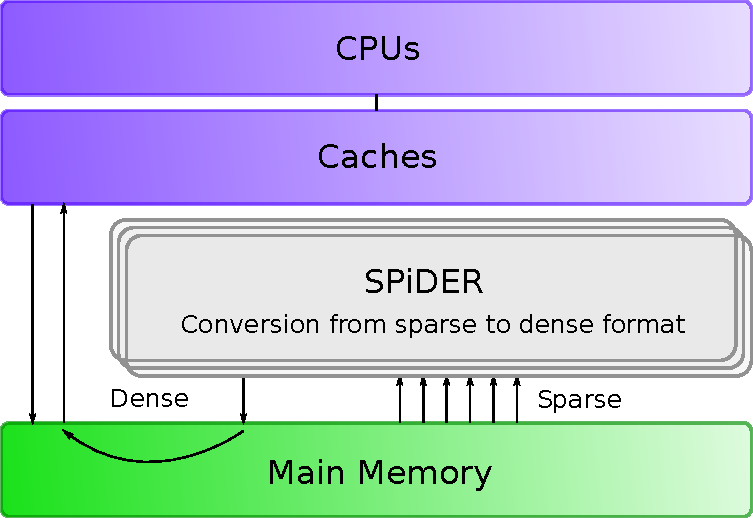
\includegraphics[width=0.49\linewidth]{Figures/PDF/SPiDRE.pdf}
    \caption{Architecture of SPiDRE}
    \label{fig:soa:spidre}
\end{figure}